% fs-12-GoodnessFit.tex

\documentclass[xcolor=dvipsnames]{beamer}
\usepackage{teachbeamer}

\title{Goodness of Fit}
\subtitle{{\CourseNumber}, BCIT}

\author{\CourseName}

\date{April 26, 2018}

% \begin{figure}[h]
% 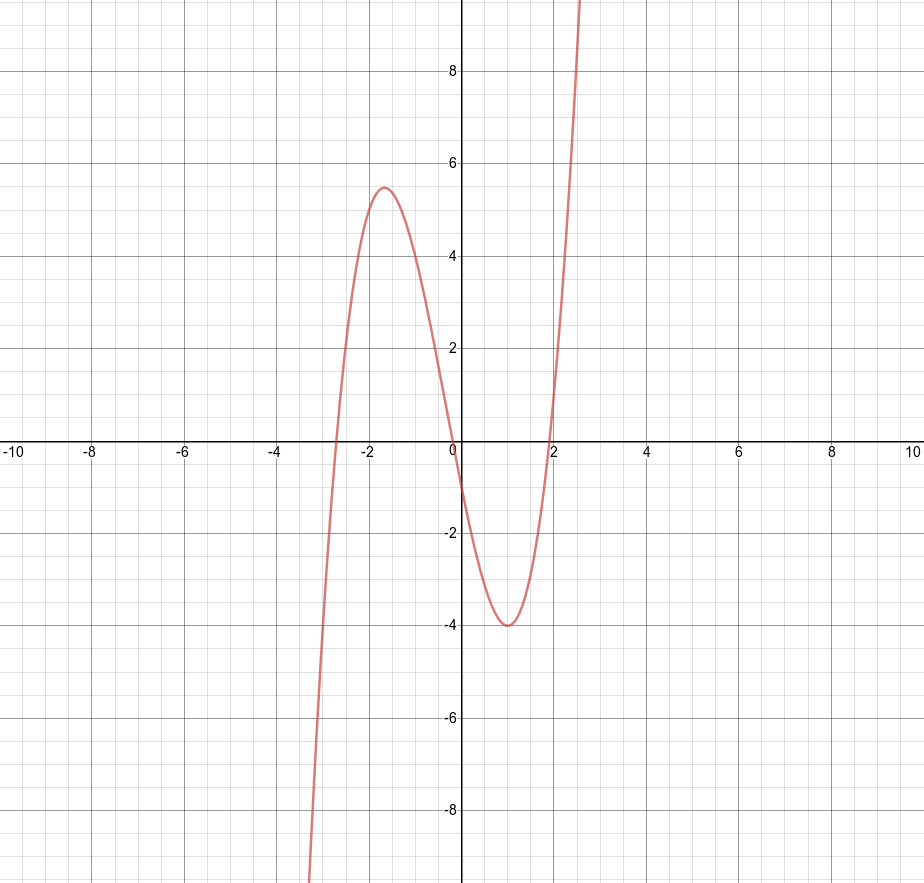
\includegraphics[scale=.3]{./diagrams/extrema1.png}
% \end{figure}

% Command             10pt    11pt    12pt
% \tiny               5       6       6
% \scriptsize         7       8       8
% \footnotesize       8       9       10
% \small              9       10      10.95
% \normalsize         10      10.95   12

\begin{document}

\begin{frame}
  \titlepage
\end{frame}

\begin{frame}
  \frametitle{Goodness of Fit}
  A \alert{goodness of fit} test is used to test the hypothesis
  that an observed frequency distribution fits (or conforms to)
  some claimed distribution.

  \begin{description}
  \item[$H_{0}$] The frequency counts agree with the claimed
    distribution.
  \item[$H_{1}$]  The frequency counts do not agree with the claimed
    distribution.
  \end{description}

  \bigskip

  \begin{block}{Test Statistic for Goodness of Fit Tests}
    $\displaystyle \chi^{2}=\sum\frac{(O-E)^{2}}{E}$
  \end{block}
\end{frame}

\begin{frame}
  \frametitle{Benford's Law}
% This LaTeX table template is generated by emacs 24.5.1
\begin{tabular}{|l|r|l|r|}
\hline
Abbotsford     & 141485 & Central Saanich & 15895  \\
\hline
Alert Bay      & 436    & Chase           & 2365   \\
\hline
Anmore         & 2322   & Chetwynd        & 2877   \\
\hline
Armstrong      & 4842   & Chilliwack      & 90390  \\
\hline
Ashcroft       & 1557   & Clearwater      & 2368   \\
\hline
Barriere       & 1751   & Clinton         & 629    \\
\hline
Belcarra       & 618    & Coldstream      & 10938  \\
\hline
Bowen Island   & 3580   & Colwood         & 17583  \\
\hline
Burnaby        & 238728 & Comox           & 14400  \\
\hline
Burns Lake     & 1803   & Coquitlam       & 147619 \\
\hline
Cache Creek    & 972    & Courtenay       & 26056  \\
\hline
Campbell River & 33696  & Cranbrook       & 20452  \\
\hline
Canal Flats    & 744    & Creston         & 4661   \\
\hline
Castlegar      & 7934   & Cumberland      & 3562   \\
\hline
\end{tabular}
% +-------------------------+-------------------------+-------------------------+-------------------------+
% |Abbotsford               |141485                   |Central Saanich          |15895                    |
% +-------------------------+-------------------------+-------------------------+-------------------------+
% |Alert Bay                |436                      |Chase                    |2365                     |
% +-------------------------+-------------------------+-------------------------+-------------------------+
% |Anmore                   |2322                     |Chetwynd                 |2877                     |
% +-------------------------+-------------------------+-------------------------+-------------------------+
% |Armstrong                |4842                     |Chilliwack               |90390                    |
% +-------------------------+-------------------------+-------------------------+-------------------------+
% |Ashcroft                 |1557                     |Clearwater               |2368                     |
% +-------------------------+-------------------------+-------------------------+-------------------------+
% |Barriere                 |1751                     |Clinton                  |629                      |
% +-------------------------+-------------------------+-------------------------+-------------------------+
% |Belcarra                 |618                      |Coldstream               |10938                    |
% +-------------------------+-------------------------+-------------------------+-------------------------+
% |Bowen Island             |3580                     |Colwood                  |17583                    |
% +-------------------------+-------------------------+-------------------------+-------------------------+
% |Burnaby                  |238728                   |Comox                    |14400                    |
% +-------------------------+-------------------------+-------------------------+-------------------------+
% |Burns Lake               |1803                     |Coquitlam                |147619                   |
% +-------------------------+-------------------------+-------------------------+-------------------------+
% |Cache Creek              |972                      |Courtenay                |26056                    |
% +-------------------------+-------------------------+-------------------------+-------------------------+
% |Campbell River           |33696                    |Cranbrook                |20452                    |
% +-------------------------+-------------------------+-------------------------+-------------------------+
% |Canal Flats              |744                      |Creston                  |4661                     |
% +-------------------------+-------------------------+-------------------------+-------------------------+
% |Castlegar                |7934                     |Cumberland               |3562                     |
% +-------------------------+-------------------------+-------------------------+-------------------------+
\end{frame}

\begin{frame}
  \frametitle{Benford's Law}
% This LaTeX table template is generated by emacs 24.5.1
\begin{tabular}{|l|r|l|r|}
\hline
Dawson Creek   & 12115  & Grand Forks          & 4029   \\
\hline
Delta          & 101997 & Granisle             & 307    \\
\hline
Duncan         & 4768   & Greenwood            & 688    \\
\hline
Elkford        & 2630   & Harrison Hot Springs & 1407   \\
\hline
Enderby        & 2815   & Hazelton             & 257    \\
\hline
Esquimalt      & 16830  & Highlands            & 2394   \\
\hline
Fernie         & 4333   & Hope                 & 5796   \\
\hline
Fort St. James & 1755   & Houston              & 3155   \\
\hline
Fort St. John  & 22618  & Hudson's Hope        & 1022   \\
\hline
Fraser Lake    & 1178   & Invermere            & 2941   \\
\hline
Fruitvale      & 2098   & Kamloops             & 91402  \\
\hline
Gibsons        & 4550   & Kaslo                & 1000   \\
\hline
Gold River     & 1254   & Kelowna              & 125737 \\
\hline
Golden         & 3862   & Kent                 & 6220   \\
\hline
\end{tabular}
% +-------------------------+-------------------------+-------------------------+-------------------------+
% |Dawson Creek             |12115                    |Grand Forks              |4029                     |
% +-------------------------+-------------------------+-------------------------+-------------------------+
% |Delta                    |101997                   |Granisle                 |307                      |
% +-------------------------+-------------------------+-------------------------+-------------------------+
% |Duncan                   |4768                     |Greenwood                |688                      |
% +-------------------------+-------------------------+-------------------------+-------------------------+
% |Elkford                  |2630                     |Harrison Hot Springs     |1407                     |
% +-------------------------+-------------------------+-------------------------+-------------------------+
% |Enderby                  |2815                     |Hazelton                 |257                      |
% +-------------------------+-------------------------+-------------------------+-------------------------+
% |Esquimalt                |16830                    |Highlands                |2394                     |
% +-------------------------+-------------------------+-------------------------+-------------------------+
% |Fernie                   |4333                     |Hope                     |5796                     |
% +-------------------------+-------------------------+-------------------------+-------------------------+
% |Fort St. James           |1755                     |Houston                  |3155                     |
% +-------------------------+-------------------------+-------------------------+-------------------------+
% |Fort St. John            |22618                    |Hudson's Hope            |1022                     |
% +-------------------------+-------------------------+-------------------------+-------------------------+
% |Fraser Lake              |1178                     |Invermere                |2941                     |
% +-------------------------+-------------------------+-------------------------+-------------------------+
% |Fruitvale                |2098                     |Kamloops                 |91402                    |
% +-------------------------+-------------------------+-------------------------+-------------------------+
% |Gibsons                  |4550                     |Kaslo                    |1000                     |
% +-------------------------+-------------------------+-------------------------+-------------------------+
% |Gold River               |1254                     |Kelowna                  |125737                   |
% +-------------------------+-------------------------+-------------------------+-------------------------+
% |Golden                   |3862                     |Kent                     |6220                     |
% +-------------------------+-------------------------+-------------------------+-------------------------+
\end{frame}

\begin{frame}
  \frametitle{Benford's Law}
% This LaTeX table template is generated by emacs 24.5.1
\begin{tabular}{|l|r|l|r|}
\hline
Keremeos           & 1348   & Lytton      & 240   \\
\hline
Kimberley          & 7050   & Mackenzie   & 3492  \\
\hline
Kitimat            & 7664   & Maple Ridge & 85653 \\
\hline
Ladysmith          & 8342   & Masset      & 859   \\
\hline
Lake Country       & 14183  & McBride     & 576   \\
\hline
Lake Cowichan      & 3169   & Merritt     & 7607  \\
\hline
Langford           & 39936  & Metchosin   & 4792  \\
\hline
Langley (city)     & 27283  & Midway      & 667   \\
\hline
Langley (district) & 122415 & Mission     & 39873 \\
\hline
Lantzville         & 3408   & Montrose    & 1020  \\
\hline
Lillooet           & 2403   & Nakusp      & 1571  \\
\hline
Lions Bay          & 1325   & Nanaimo     & 93351 \\
\hline
Logan Lake         & 2099   & Nelson      & 11249 \\
\hline
Lumby              & 1772   & New Denver  & 519   \\
\hline
\end{tabular}
% +-------------------------+-------------------------+-------------------------+-------------------------+
% |Keremeos                 |1348                     |Lytton                   |240                      |
% +-------------------------+-------------------------+-------------------------+-------------------------+
% |Kimberley                |7050                     |Mackenzie                |3492                     |
% +-------------------------+-------------------------+-------------------------+-------------------------+
% |Kitimat                  |7664                     |Maple Ridge              |85653                    |
% +-------------------------+-------------------------+-------------------------+-------------------------+
% |Ladysmith                |8342                     |Masset                   |859                      |
% +-------------------------+-------------------------+-------------------------+-------------------------+
% |Lake Country             |14183                    |McBride                  |576                      |
% +-------------------------+-------------------------+-------------------------+-------------------------+
% |Lake Cowichan            |3169                     |Merritt                  |7607                     |
% +-------------------------+-------------------------+-------------------------+-------------------------+
% |Langford                 |39936                    |Metchosin                |4792                     |
% +-------------------------+-------------------------+-------------------------+-------------------------+
% |Langley (city)           |27283                    |Midway                   |667                      |
% +-------------------------+-------------------------+-------------------------+-------------------------+
% |Langley (district)       |122415                   |Mission                  |39873                    |
% +-------------------------+-------------------------+-------------------------+-------------------------+
% |Lantzville               |3408                     |Montrose                 |1020                     |
% +-------------------------+-------------------------+-------------------------+-------------------------+
% |Lillooet                 |2403                     |Nakusp                   |1571                     |
% +-------------------------+-------------------------+-------------------------+-------------------------+
% |Lions Bay                |1325                     |Nanaimo                  |93351                    |
% +-------------------------+-------------------------+-------------------------+-------------------------+
% |Logan Lake               |2099                     |Nelson                   |11249                    |
% +-------------------------+-------------------------+-------------------------+-------------------------+
% |Lumby                    |1772                     |New Denver               |519                      |
% +-------------------------+-------------------------+-------------------------+-------------------------+
\end{frame}

\begin{frame}
  \frametitle{Benford's Law}
% This LaTeX table template is generated by emacs 24.5.1
\begin{tabular}{|l|r|l|r|}
\hline
New Hazelton               & 642   & Penticton      & 33016 \\
\hline
New Westminster            & 73771 & Pitt Meadows   & 19090 \\
\hline
North Cowichan             & 30229 & Port Alberni   & 16236 \\
\hline
North Saanich              & 11143 & Port Alice     & 785   \\
\hline
North Vancouver (city)     & 52794 & Port Clements  & 366   \\
\hline
North Vancouver (district) & 86602 & Port Coquitlam & 61187 \\
\hline
Northern Rockies           & 5384  & Port Edward    & 474   \\
\hline
Oak Bay                    & 17368 & Port Hardy     & 3731  \\
\hline
Oliver                     & 4568  & Port McNeill   & 2500  \\
\hline
One Hundred Mile House     & 1860  & Port Moody     & 34193 \\
\hline
Osoyoos                    & 4800  & Pouce Coupe    & 689   \\
\hline
Parksville                 & 12883 & Powell River   & 13729 \\
\hline
Peachland                  & 4959  & Prince George  & 70912 \\
\hline
Pemberton                  & 2511  & Prince Rupert  & 11261 \\
\hline
\end{tabular}
% +-------------------------+-------------------------+-------------------------+-------------------------+
% |New Hazelton             |642                      |Penticton                |33016                    |
% +-------------------------+-------------------------+-------------------------+-------------------------+
% |New Westminster          |73771                    |Pitt Meadows             |19090                    |
% +-------------------------+-------------------------+-------------------------+-------------------------+
% |North Cowichan           |30229                    |Port Alberni             |16236                    |
% +-------------------------+-------------------------+-------------------------+-------------------------+
% |North Saanich            |11143                    |Port Alice               |785                      |
% +-------------------------+-------------------------+-------------------------+-------------------------+
% |North Vancouver (city)   |52794                    |Port Clements            |366                      |
% +-------------------------+-------------------------+-------------------------+-------------------------+
% |North Vancouver          |86602                    |Port Coquitlam           |61187                    |
% |(district)               |                         |                         |                         |
% +-------------------------+-------------------------+-------------------------+-------------------------+
% |Northern Rockies Regional|5384                     |Port Edward              |474                      |
% |Municipality             |                         |                         |                         |
% +-------------------------+-------------------------+-------------------------+-------------------------+
% |Oak Bay                  |17368                    |Port Hardy               |3731                     |
% +-------------------------+-------------------------+-------------------------+-------------------------+
% |Oliver                   |4568                     |Port McNeill             |2500                     |
% +-------------------------+-------------------------+-------------------------+-------------------------+
% |One Hundred Mile House   |1860                     |Port Moody               |34193                    |
% +-------------------------+-------------------------+-------------------------+-------------------------+
% |Osoyoos                  |4800                     |Pouce Coupe              |689                      |
% +-------------------------+-------------------------+-------------------------+-------------------------+
% |Parksville               |12883                    |Powell River             |13729                    |
% +-------------------------+-------------------------+-------------------------+-------------------------+
% |Peachland                |4959                     |Prince George            |70912                    |
% +-------------------------+-------------------------+-------------------------+-------------------------+
% |Pemberton                |2511                     |Prince Rupert            |11261                    |
% +-------------------------+-------------------------+-------------------------+-------------------------+
\end{frame}

\begin{frame}
  \frametitle{Benford's Law}
% This LaTeX table template is generated by emacs 24.5.1
\begin{tabular}{|l|r|l|r|}
\hline
Princeton              & 2782   & Sechelt (Sunshine Coast) & 21     \\
\hline
Qualicum Beach         & 8687   & Sicamous                 & 2468   \\
\hline
Queen Charlotte        & 943    & Sidney                   & 11129  \\
\hline
Quesnel                & 9026   & Silverton                & 199    \\
\hline
Radium Hot Springs     & 764    & Slocan                   & 309    \\
\hline
Revelstoke             & 7316   & Smithers                 & 5462   \\
\hline
Richmond               & 213392 & Sooke                    & 11868  \\
\hline
Rossland               & 3639   & Spallumcheen             & 5222   \\
\hline
Saanich                & 110889 & Sparwood                 & 4078   \\
\hline
Salmo                  & 1165   & Squamish                 & 19067  \\
\hline
Salmon Arm             & 18128  & Stewart                  & 423    \\
\hline
Sayward                & 311    & Summerland               & 11375  \\
\hline
Sechelt Municipality   & 9490   & Sun Peaks Mountain       & 457    \\
\hline
Sechelt (Powell River) & 831    & Surrey                   & 543940 \\
\hline
\end{tabular}
% +-------------------------+-------------------------+-------------------------+-------------------------+
% |Princeton                |2782                     |Sechelt (Sunshine Coast) |21                       |
% +-------------------------+-------------------------+-------------------------+-------------------------+
% |Qualicum Beach           |8687                     |Sicamous                 |2468                     |
% +-------------------------+-------------------------+-------------------------+-------------------------+
% |Queen Charlotte          |943                      |Sidney                   |11129                    |
% +-------------------------+-------------------------+-------------------------+-------------------------+
% |Quesnel                  |9026                     |Silverton                |199                      |
% +-------------------------+-------------------------+-------------------------+-------------------------+
% |Radium Hot Springs       |764                      |Slocan                   |309                      |
% +-------------------------+-------------------------+-------------------------+-------------------------+
% |Revelstoke               |7316                     |Smithers                 |5462                     |
% +-------------------------+-------------------------+-------------------------+-------------------------+
% |Richmond                 |213392                   |Sooke                    |11868                    |
% +-------------------------+-------------------------+-------------------------+-------------------------+
% |Rossland                 |3639                     |Spallumcheen             |5222                     |
% +-------------------------+-------------------------+-------------------------+-------------------------+
% |Saanich                  |110889                   |Sparwood                 |4078                     |
% +-------------------------+-------------------------+-------------------------+-------------------------+
% |Salmo                    |1165                     |Squamish                 |19067                    |
% +-------------------------+-------------------------+-------------------------+-------------------------+
% |Salmon Arm               |18128                    |Stewart                  |423                      |
% +-------------------------+-------------------------+-------------------------+-------------------------+
% |Sayward                  |311                      |Summerland               |11375                    |
% +-------------------------+-------------------------+-------------------------+-------------------------+
% |Sechelt Municipality     |9490                     |Sun Peaks Mountain       |457                      |
% +-------------------------+-------------------------+-------------------------+-------------------------+
% |Sechelt (Powell River)   |831                      |Surrey                   |543940                   |
% +-------------------------+-------------------------+-------------------------+-------------------------+
\end{frame}

\begin{frame}
  \frametitle{Benford's Law}
% This LaTeX table template is generated by emacs 24.5.1
\begin{tabular}{|l|r|l|r|}
\hline
Tahsis        & 295    & Warfield       & 1669  \\
\hline
Taylor        & 1544   & Wells          & 231   \\
\hline
Telkwa        & 1328   & West Kelowna   & 34930 \\
\hline
Terrace       & 10659  & West Vancouver & 40923 \\
\hline
Tofino        & 2190   & Whistler       & 10627 \\
\hline
Trail         & 7376   & White Rock     & 19288 \\
\hline
Tumbler Ridge & 2853   & Williams Lake  & 11028 \\
\hline
Ucluelet      & 1634   & Zeballos       & 99    \\
\hline
Valemount     & 947    & Wells          & 231   \\
\hline
Vancouver     & 653046 & West Kelowna   & 34930 \\
\hline
Vanderhoof    & 4526   & West Vancouver & 40923 \\
\hline
Vernon        & 41671  & Whistler       & 10627 \\
\hline
Victoria      & 85192  & White Rock     & 19288 \\
\hline
View Royal    & 10137  & Williams Lake  & 11028 \\
\hline
Warfield      & 1669   & Zeballos       & 99    \\
\hline
\end{tabular}
% +-------------------------+-------------------------+-------------------------+-------------------------+
% |Tahsis                   |295                      |Warfield                 |1669                     |
% +-------------------------+-------------------------+-------------------------+-------------------------+
% |Taylor                   |1544                     |Wells                    |231                      |
% +-------------------------+-------------------------+-------------------------+-------------------------+
% |Telkwa                   |1328                     |West Kelowna             |34930                    |
% +-------------------------+-------------------------+-------------------------+-------------------------+
% |Terrace                  |10659                    |West Vancouver           |40923                    |
% +-------------------------+-------------------------+-------------------------+-------------------------+
% |Tofino                   |2190                     |Whistler                 |10627                    |
% +-------------------------+-------------------------+-------------------------+-------------------------+
% |Trail                    |7376                     |White Rock               |19288                    |
% +-------------------------+-------------------------+-------------------------+-------------------------+
% |Tumbler Ridge            |2853                     |Williams Lake            |11028                    |
% +-------------------------+-------------------------+-------------------------+-------------------------+
% |Ucluelet                 |1634                     |Zeballos                 |99                       |
% +-------------------------+-------------------------+-------------------------+-------------------------+
% |Valemount                |947                      |Wells                    |231                      |
% +-------------------------+-------------------------+-------------------------+-------------------------+
% |Vancouver                |653046                   |West Kelowna             |34930                    |
% +-------------------------+-------------------------+-------------------------+-------------------------+
% |Vanderhoof               |4526                     |West Vancouver           |40923                    |
% +-------------------------+-------------------------+-------------------------+-------------------------+
% |Vernon                   |41671                    |Whistler                 |10627                    |
% +-------------------------+-------------------------+-------------------------+-------------------------+
% |Victoria                 |85192                    |White Rock               |19288                    |
% +-------------------------+-------------------------+-------------------------+-------------------------+
% |View Royal               |10137                    |Williams Lake            |11028                    |
% +-------------------------+-------------------------+-------------------------+-------------------------+
% |Warfield                 |1669                     |Zeballos                 |99                       |
% +-------------------------+-------------------------+-------------------------+-------------------------+
\end{frame}

\begin{frame}
  \frametitle{Benford's Law}
  The distribution of first digits is as follows:
  \begin{tabular}{|r|r|r|r|r|r|r|r|r|}\hline
   1 & 2 & 3 & 4 & 5 & 6 &  7 & 8 & 9 \\ \hline
   52 & 28 & 20 & 18 & 8 & 9 & 11 & 7 &  9 \\ \hline
  \end{tabular}

\bigskip

  Now let's see if this is consistent with a uniform distribution.

\bigskip

\begin{footnotesize}
  \begin{tabular}{|l|r|r|r|r|r|r|r|r|r|}\hline
                 & 1    & 2    & 3    & 4    & 5     & 6     & 7     & 8     & 9     \\ \hline
   $O$           & 52   & 28   & 20   & 18   & 8     & 9     & 11    & 7     & 9     \\ \hline
   $E$           & 18   & 18   & 18   & 18   & 18    & 18    & 18    & 18    & 18    \\ \hline
   $O-E$         & 34   & 10   & 2    & 0    & -10   & -9    & -7    & -11   & -9    \\ \hline
   $(O-E)^{2}$   & 1156 & 100  & 4    & 0    & 100   & 81    & 49    & 121   & 81    \\ \hline
   $(O-E)^{2}/E$ & 64.22 & 5.56 & 0.22 & 0.00 & 5.56 & 4.50 & 2.72 & 6.72 & 4.50 \\ \hline
  \end{tabular}
\end{footnotesize}

\bigskip

The sum of the last row is $94$. The degree of freedom is $8$ (the
degree of freedom is $k-1$, where $k$ is the number of categories,
\emph{not} the sample size $n$). Consulting the Chi-Square
$\chi^{2}$ Distribution table, we record the critical value as
$15.507$, using $\alpha=0.05$. We reject the null hypothesis.
\end{frame}

\begin{frame}
  \frametitle{Benford's Law}
  A set of numbers is said to satisfy Benford's law if the leading digit $d$ ($d\in\{1,{\ldots},9\}$) occurs with probability
  \begin{equation}
    \label{eq:aihuwoob}
    P(d)=\log_{10}(d+1)-\log_{10}(d)=\log_{10}\left(1+\frac{1}{d}\right)
  \end{equation}
\end{frame}

\begin{frame}
  \frametitle{Benford's Law}
  The distribution of first digits is as follows:
  \begin{tabular}{|r|r|r|r|r|r|r|r|r|}\hline
   1 & 2 & 3 & 4 & 5 & 6 &  7 & 8 & 9 \\ \hline
   52 & 28 & 20 & 18 & 8 & 9 & 11 & 7 &  9 \\ \hline
  \end{tabular}

\bigskip

  Now let's see if this is consistent with Benford's Law.

\bigskip

\begin{scriptsize}
  \begin{tabular}{|l|r|r|r|r|r|r|r|r|r|}\hline
                 & 1     & 2     & 3     & 4    & 5     & 6     & 7    & 8     & 9    \\ \hline
   $O$           & 52    & 28    & 20    & 18   & 8     & 9     & 11   & 7     & 9    \\ \hline
   $E$           & 48.8  & 28.5  & 20.2  & 15.7 & 12.8  & 10.8  & 9.4  & 8.3   & 7.4  \\ \hline
   $O-E$         & 3.23  & -0.53 & -0.24 & 2.30 & -4.83 & -1.85 & 1.61 & -1.29 & 1.59 \\ \hline
   $(O-E)^{2}$   & 10.45 &  0.28 &  0.06 &  5.29 & 23.30 & 3.41 & 2.58 & 1.66 & 2.52 \\ \hline
   $(O-E)^{2}/E$ & 0.58 & 0.015 & 0.0032 & 0.29 & 1.29 & 0.19 & 0.14 & 0.09 & 0.14 \\ \hline
  \end{tabular}
\end{scriptsize}

\bigskip

The sum of the last row is $3.508727$, which is also the test
statistic. The critical value is still $\chi^{2}=15.507$. We fail
to reject the null hypothesis.
\end{frame}

\begin{frame}[fragile]
  \frametitle{R Commands for Goodness of Fit Test}
\begin{alltt}
o<-c(52,28,20,18,8,9,11,7,9) \newline
s<-seq(1,9,1) \newline
bf<-log(1+(1/s))/log(10) \newline
e<-bf*162 \newline
chisq.test(o,p=bf)
\end{alltt}
\end{frame}

% 6.	Last Digits of Heights Example 1 in this section involved an analysis of the last digits of weights from a random sample of 100 Californians. Using those same subjects, the last digits of their heights arc listed in the table below (based on data from the California Department of Public Health). Use a 0.05 significance level to test the claim that the sample is from a population of heights in which the last digits do not occur with the same frequency. The accompanying Minitab display results from the data in the table.
% Last Digit	0	1	2	3	4	5	6	7	8	9	
% 											M df Chi-Sq P-Value 100 9 6. 6 0.679
% Frequency	12	8	14	9	11	9	13	8	11	5	

\begin{frame}
  \frametitle{Goodness of Fit Exercises}
  {\ubung} Mario Triola purchased a slot machine (Bally Model 809) and
  tested it by playing it 1197 times. There are 10 different
  categories of outcomes, including no win, win jackpot, win with
  three bells, and so on. When testing the claim that the observed
  outcomes agree with the expected frequencies, the author obtained a
  test statistic of $\chi^{2}=8.185$. Use a 0.05 significance level to
  test the claim that the actual outcomes agree with the expected
  frequencies. Does the slot machine appear to be functioning as
  expected?
\end{frame}

\begin{frame}
  \frametitle{Goodness of Fit Exercises}
  {\ubung} For a recent year, the following are the numbers of
  homicides that occurred each month in New York City: 38, 30, 46, 40,
  46, 49, 47, 50, 50, 42, 37, 37. Use a 0.05 significance level to
  test the claim that homicides in New York City are equally likely
  for each of the 12 months. Is there sufficient evidence to support
  the police commissioner's claim that homicides occur more often in
  the summer when the weather is better?
\end{frame}

% 8.	Flat Tiro and Missed Class A classic story' involves four carpooling students who missed a test and gave as an excuse a flat tire. On the makeup test, the instructor asked the students to identify the particular lire that went flat. If they really didn’t have a flat tire, would they be able to identify the same tire? The author asked 41 other students to identify the tire they would select. The results arc listed in the following table (except for one student who selected the spare). Use a 0.05 significance Icsel to test the author’s claim that the results fit a uniform distribution. What docs the result suggest about the ability of the four students to select the same tire when they really didn’t have a flat?
% Tire	Lett Front	Right Front	Left Rear	Right Rear
% Number Selected	11	15	8	6

\begin{frame}
  \frametitle{Goodness of Fit Exercises}
  {\ubung} In his book \emph{Outliers}, author Malcolm Gladwell argues
  that more baseball players have birthdates in the months immediately
  following July 31, because that was the cutoff date for nonschool
  baseball leagues. Here is a sample of frequency counts of months of
  birthdates of American-born major league baseball players starting
  with January: 387, 329, 366, 344, 336, 313, 313, 503, 421,434, 398,
  371. Using a 0.05 significance level, is there sufficient evidence
  to warrant rejection of the claim that American-born major league
  baseball players are born in different months with the same
  frequency? Do the sample values appear to support Gladwell's claim?
\end{frame}

\begin{frame}
  \frametitle{Goodness of Fit Exercises}
  {\ubung} Mario Triola drilled a hole in a die and filled it with a
  lead weight, then proceeded to roll it 200 times. Here are the
  observed frequencies for the outcomes of 1, 2, 3, 4, 5, and 6,
  respectively: 27, 31, 42, 40, 28, 32. Use a 0.05 significance level
  to test the claim that the outcomes are not equally likely. Does it
  appear that the loaded die behaves differently than a fair die?
\end{frame}

\begin{frame}[fragile]
  \frametitle{Goodness of Fit Exercises}
  {\ubung} Records of randomly selected births were obtained and
  categorized according to the day of the week that they occurred
  (based on data from the National Center for Health Statistics).
  Because babies are unfamiliar with our schedule of weekdays, a
  reasonable claim is that births occur on the different days with
  equal frequency. See the table that follows. Use a 0.01 significance
  level to test that claim. Can you provide an explanation for the
  result?
\begin{verbatim}
+------+------+------+------+------+------+------+------+
|Day   |Sun   |Mon   |Tue   |Wed   |Thu   |Fri   |Sat   |
+------+------+------+------+------+------+------+------+
|Number|77    |110   |124   |122   |120   |123   |97    |
+------+------+------+------+------+------+------+------+
\end{verbatim}
\end{frame}

\begin{frame}
  \frametitle{Goodness of Fit Exercises}
  {\ubung} Do World War II Bomb Hits Fit a Poisson Distribution?
  In analyzing hits by V-1 buzz bombs in World War II, South
  London was subdivided into regions, each with an area of 0.25
  km$^{2}$. Shown below is a table of actual frequencies of hits
  and the frequencies expected with the Poisson distribution
  (first row: Number of Bomb Hits; second row: Actual Number of
  Regions; third row: Expected Number of Regions from Poisson
  Distribution). Use the values listed and a 0.05 significance
  level to test the claim that the actual frequencies fit a
  Poisson distribution.

  \medskip

\begin{tabular}{|r|r|r|r|r|}\hline
\textbf{0} & \textbf{1} & \textbf{2} & \textbf{3} & \textbf{4} \\ \hline
229        & 211        & 93         & 35         & 8          \\ \hline
227.5      & 211.4      & 97.9       & 30.5       & 8.7        \\ \hline
\end{tabular}
\end{frame}

% 13.	Kentucky Derby Ilie table below lists the frequency of wins for different post positions in the Kentucky Derby horse race (current as of this writing). A post position of 1 is closest to the inside rail, so that horse has the shortest distance to run. (Because the number of horses varies from year to year, only the first 10 post positions are included.) Use a 0.05 significance level to test the claim that the likelihood of winning is the same for the different post positions. Based on the result, should bettors consider the post position of a horse racing in the Kentucky Derby?
% Post Position	1	2	3	4	5	6	7	8	9	10
% Wins	19	14	11	15	14	7	8	12	5	11
% 14.	Win 4 Lottery The author recorded all digits selected in New York’s Win 4 Lottery for two drawings held each day in a recent year. The frequencies of the digits from 0 through 9 are 280, 303. 331, 289, 285, 294. 283, 274, 297, and 284. Use a 0.05 significance level to test the claim of lottery officials that the digits arc selected in a way that they arc equally likely.
% 15.	Police Calls 'Die police depan man in Madison, Connecticut, released the following numbers of calls for the different days of the week during a recent February that had 28 days: Monday (114); Tuesday (152); Wednesday (160); Thursday (164); Friday (179); Saturday (1%); Sunday (130). Use a 0.01 significance level to test the claim that the different days of the week have the same frequencies of police calls. Is there anything notable about the observed frequencies?
% 16.	Police Calls Repeat the preceding exercise using these observed frequencies for police calls received during the month of March: Monday (208); Tuesday (224); Wednesday (246); Thursday ( 173); Friday (210); Saturday (236); Sunday ( 154). What is a fundamental error with this analysis?
% 17.	World Series Games The table below lists the numbers of games played in the baseball World Series as of this writing. That table also includes the expected proportions for the numbers of games in a World Series, assuming that in each series, both teams have about the same chance of winning. Use a 0.05 significance level to test the claim that the actual numbers of games fit the distribution indicated by the expected proportions.
% Games Played	4	5	6	7
% Actual World Series Contests	20	23	23 I	37
% Expected Proportion	2/16	4/16	5/16	5/16
% 18.	American Idol The contestants on the TV show American Idol try to win a singing contest. At one point, the Web site WhatNot l oSing.com listed the actual numbers of eliminations for different orders of singing, and the expected number of eliminations was also listed. The results arc in the table below. Use a 0.05 significance level to test the claim that the actual eliminations agree with the expected numbers. Docs there appear to Ik support for the claim that the Icadoff singers appear to be at a disadvantage?
% Singing Order	1	2	3	4	5	6	7 through 12
% Eliminations	20	12	9	8	6	5	9
% Expected Eliminations	12 9	129	99	7.9	6.4 I	5.5	13.5
% 19.	M&M Candies Mars. Inc. claims that its M&M plain candies arc distributed with the following color percentages: 16% green, 20% orange, 14% yellow, 24% blue. 13% red, and 13% brown. Refer to Data Set 20 in Appendix B and use the sample data to test the claim that the color distribution is as claimed by Mars, Inc. Use a 0.05 significance level.
% Benford’s Imw. According to Benford’s law, a variety of different data sets include numbers with leading (first) digits that follow the distribution shown in the table below. In Exercises 21-24, test for goodness-of-fit with Benford's law.
% Leading Digit	1 2	3	4	5	6	7	8	9
% Benford's Lav.1: Distribution of Leading Digits	30.1% 17.6%	12.5%	9.7%	7.9%	6.7%	5.8%	5.1%	4.6%
% 21.	Detecting Fraud When working for the Brooklyn district attorney, investigator Robert Burton analyzed the leading digits of the amounts from 784 checks issued by seven suspect companies. The frequencies were found to be 0, 15, 0, 76, 479, 183, 8, 23, and 0. and those digits correspond to the leading digits of 1, 2, 3, 4, 5, 6, 7, 8, and 9, respectively. If the observed frequencies are substantially different from the frequencies expected with Benford’s law, the check amounts appear to result from fraud. Use a 0.01 significance level to test for goodness-of-fit with Benford’s law. Does it appear that the checks arc the result of fraud?
% 22.	Author’s Check Amounts Exercise 21 lists the observed frequencies of leading digits from amounts on checks from seven suspect companies. Here are the observed frequencies of the leading digits from the amounts on checks written by the author: 68, 40, 18, 19, 8, 20, 6, 9, 12. (Those observed frequencies correspond to the leading digits of 1, 2, 3, 4, 5, 6, 7, 8, and 9, respectively.) Using a 0.05 significance level, test the claim that these leading digits arc from a population of leading digits that conform to Benford’s law. Do the author’s check amounts appear to be legitimate?
% 23.	Tax Cheating? Frequencies of leading digits from 1RS tax files arc 152, 89, 63, 48, 39, 40, 28, 25, and 27 (corresponding to the leading digits of 1, 2, 3, 4, 5, 6, 7, 8. and 9, respectively, based on data from Mark Nigrini, who sells software for Benford data analysis). Using a 0.05 significance level, test for goodness-of-fit with Benford’s law. Does it appear that the tax entries arc legitimate?
% 24.	Author’s Computer Files The author recorded the leading digits of the sizes of the files stored on his computer, and the leading digits have frequencies of 45, 32, 18, 12, 9, 3, 13, 9, and 9 (corresponding to the leading digits of 1, 2, 3, 4, 5, 6, 7, 8, and 9, respectively). Using a 0.05 significance level, test for goodness-of-fit with Benford’s law.

\begin{frame}
  \frametitle{Contingency Tables}
  A \alert{contingency table} is a table consisting of frequency
  counts of categorical data corresponding to two different
  variables.

  \bigskip

  In a \alert{test of independence}, we test the null hypothesis
  that in a contingency table, the row and column variables are
  independent. (That is, there is no dependency between the row
  variable and the column variable.)
\end{frame}

\begin{frame}[fragile]
  \frametitle{Test of Independence}
  \beispiel{Smoking Cessation} The accompanying table summarizes
  successes and failures when subjects used different methods
  when trying to stop smoking. The determination of smoking or not
  smoking was made five months after the treatment was begun, and
  the data are based on results from the Centers for Disease
  Control and Prevention. Test the claim that success is
  independent of the method used at a significance level of 0.05.
  % If we test the claim that success is
  % independent of the method used, the ‘1*1-83/84 Plus calculator
  % provides a lvalue of 0.216 (rounded). What docs the /’-value
  % tell us about that claim?
\begin{verbatim}
+------------+------+-------+---------+
|Nicotine    |Gum   |Patch  |Inhaler  |
+------------+------+-------+---------+
|Smoking     |191   |263    |95       |
+------------+------+-------+---------+
|Not Smoking |59    |57     |27       |
+------------+------+-------+---------+
\end{verbatim}
% Nicotine Gum,Nicotine Patch,Nicotine Inhaler
% Smoking,191,263,95
% Not Smoking,59,57,27
\end{frame}

\begin{frame}
  \frametitle{Test of Independence}
  Let $O$ be the observed frequencies; $E$ the expected
  frequencies; $r$ represents the number of rows, $c$ the number
  of columns. The requirements are as follows:
  \begin{enumerate}
  \item The sample data are randomly selected.
  \item The sample data are represented as frequency counts in a
    two-way table.
  \item For every cell in the contingency table, the expected
    frequency $E$ is at least 5.
  \end{enumerate}
\end{frame}

\begin{frame}
  \frametitle{Test of Independence}
  The null hypothesis is that the row and column variables are
  independent. The test statistic is
  \begin{equation}
    \label{eq:eikaecee}
    \chi^{2}=\sum\frac{(O-E)^{2}}{E}
  \end{equation}
  The expected values are
  \begin{equation}
    \label{eq:anairieb}
    E=\frac{\mbox{(row total)(column total)}}{\mbox{(grand total)}}
  \end{equation}
Use degree of freedom $(r-1)\cdot{}(c-1)$.
\end{frame}

\begin{frame}
  \frametitle{Test of Independence}
  \begin{figure}[h]
    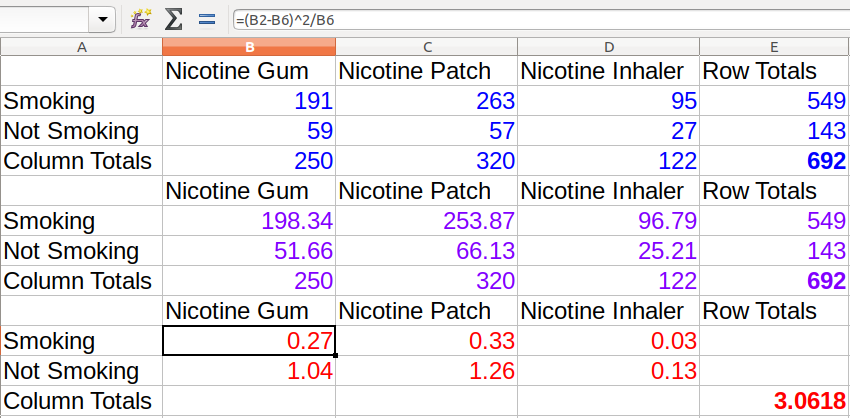
\includegraphics[scale=0.35]{./diagrams/conttable.png}
  \end{figure}
\end{frame}

% Statistical Literacy and Critical Thinking
% 2.	Terminology I he table in Exercise 1 is called a contingency table or two-way table. Why is the term contingency used? Why is the terminology of two-way table used?
% 3.	Degrees of Freedom and Critical Value For the hypothesis test in Exercise 1. the test statistic is 3.062. Find the number of degrees of freedom used to find the critical value, then find the critical value. Assume a 0.05 significance level.
% 4.	Right-Tailed, Left-Tailed, Two-Tailed Is the hypothesis test in Exercise 1 right-tailed, left-tailed, or two-tailed? Explain your choice.
% In Exercises 5-18, test the given claim.
% 5.	Denomination Effect In a study of the “denomination effect" described in the Chapter Problem, 150 women in China were given either a single 100 Yuan bill or a total of 100 Yuan in smaller bills. I*he value of 100 Yuan is about $15. The women were given the choice of spending the money on specific items or the)’ could keep the money. The results are summarized in the table below, and STATDISK results are provided in the screen display. Use a 0.05 significance loci to test the claim that the form of the 100 Yuan is independent of whether the money was spent. What docs the result suggest about a denomination effect?
% 	Spent the Money	Kept the Money
% Women Given a Smgte 100-Yuan Bin	60 68	15
% Women Given 100 Yuan in Smaller Bills		7
% 6. Which Treatment Is Better? A randomized controlled trial was designed to compare the effectiveness of splinting versus surgery in the treatment of carpal tunnel syndrome. Results arc given in the table below (based on data from “Splinting vs. Surgery in the Treatment of Carpal Tunnel Syndrome." by Gerritsen ct al .Journal oftlx American Medical Association, Vol. 288. No. 10). The results arc based on evaluations made one year after the treatment. Minitab results are given below the table. Using a 0.01 significance level, test the claim that success is independent of the type of treatment. What do the results suggest about treating carpal tunnd syndrome?
% 	Successful Treatment	Unsuccessful Treatment
% Splint Treatment	60	23
% Surgery Treatment	67	6
% MINITAB
% C-hi-Sq - 9.7SO, DF - 1, P-Valu* - 0 002

\begin{frame}
  \frametitle{Test of Independence Exercise}
  {\ubung} The table below includes results from polygraph (lie
  detector) experiments conducted by researchers Charles R. Honts
  (Boise State University) and Gordon H. Barland (Department of Defense
  Polygraph Institute). In each ease, it was known if the subject lied
  or did not lie, so the table indicates when the polygraph test was
  correct. Use a 0.05 significance level to test the claim that
  whether a subject lies is independent of the polygraph test
  indication. Do the results suggest that polygraphs are effective in
  distinguishing between truths and lies?

  \bigskip
  
  \begin{tabular}{|l|c|c|}\hline
    & subject did not lie & subject lied \\ \hline
    polygraph indicated lie & 15 & 42 \\ \hline
    polygraph indicated no lie & 32 & 9 \\ \hline
  \end{tabular}
\end{frame}

% 8. Discrimination The U.S. Supreme Court considered a ease involving the exam for firefighter lieutenant in the city of New’ Haven, Connecticut. Results from the exam arc shown in the table below. Is there sufficient evidence to support the claim that results from the test should be thrown out because they arc discriminatory? Use a 0.01 significance level.	&
% 	Passed	Failed
% White Candidates	17	16
% Minority Candidates	9	25
% 9. Is Sentence Independent of Plea? Many people believe that criminals who plead guilty tend to get lighter sentences than those who are convicted in trials. The accompanying table summarizes randomly selected sample data for San Francisco defendants in burglary cases (based on data from “Does It Pay to Plead Guilty? Differential Sentencing and the Functioning O' ,,lc ^nmmal Coiirw.” by Brcrcton and Casper, Law and Society Review, Vol. 16, No. 1). All of the subjects had prior prison sentences. Use a 0.05 significance level to test the claim that die rentcncc (sent to prison or not sent to prison) is independent of the plea. If you were an attorney defending a guilty defendant, w'ould these results suggest that you should encourage a guilty plea?
% Guilty Plea		Not Guilty Plea
% Sent to Prison	392	58
% Not Sent to Prison	564	14

\begin{frame}
  \frametitle{Test of Independence Exercise}
  {\ubung} Alert nurses at the Veteran's Affairs Medical Centre in
  Northampton, Massachusetts, noticed an unusually high number of
  deaths at times when another nurse, Kristen Gilbert, was working.
  Those same nurses later noticed missing supplies of the drug
  epinephrine, which is a synthetic adrenaline that stimulates the
  heart. Kristen Gilbert was arrested and charged with four counts of
  murder and two counts of attempted murder. When seeking a grand jury
  indictment, prosecutors provided a key piece of evidence consisting
  of the table below. Use a 0.01 significance levd to test the
  defence claim that deaths on shifts are independent of whether
  Gilbert was working. What does the result suggest about the guilt or
  innocence of Gilbert?

  \bigskip

  \begin{tabular}{|l|c|c|}\hline
                    & shifts with death & shifts w/o death \\ \hline
Gilbert working     & 40                & 217              \\ \hline
Gilbert not working & 34                & 1350             \\ \hline
  \end{tabular}
\end{frame}

\begin{frame}[fragile]
  \frametitle{Test of Independence Exercise}
  {\ubung} Each one of a large population of objects has the following two
  properties: shape (circular, square, hexagonal, cross) and colour
  (green, yellow, red, blue). Do shape and colour depend on each
  other? Use the following sample data of 591 objects and a 10\%
  significance level. The data is provided as a comma-separated values
  (CSV) table for easy import into Microsoft Excel.
\begin{verbatim}
,circular,square,hexagonal,cross,
green,57,44,7,23,131
yellow,25,23,18,83,149
red,68,48,32,4,152
blue,47,7,51,54,159
,197,122,108,164,591
\end{verbatim}
\end{frame}

% 11.	Tennis Challenges Ilic table below shows results sincuv2006 of challenged referee calls In the U.S. Open. Use a 0.05 significance level to less the claim (has the gender of she tennis player is independent of whether the call is overturned.
% Yoa	No
% Men 42i	991
% Women 220	539
% 12. Lefties A random sample of760 subjects was obtained, and each was tested for left-hand writing. Results arc in the table below (based on data from “The Left-Handed: Their Sinister 1 liscory. by Elaine bowler (kiscas. Education Resources Information (xrnicr. Paper 399519). Use a 0.05 significance level to rest the claim that left-handedness is independent of gender.	
% Was the Challenge to the Call Successful?
% 	Wrrioswilh Loft Hand?	
% 	Yes	NO
% Malo	23	217
% Fomato	65	455

\begin{frame}
  \frametitle{Test of Independence Exercise}
  {\ubung} In soccer, serious fouls result in a penalty kick with one
  kicker and one defending goalkeeper. The table below summarizes
  results from 286 kicks during games among top teams.
  % (based on data
  % from ``Action Bias Among Elite Soccer Goalkeepers: The Case of
  % Penalty Kicks, by Bar-Eli et al. Journal of Economic Psychology,
  % Vol.\ 28, No.\ 5).
  In the table, jump direction indicates which way
  the goalkeeper jumped, where the kick direction is from the
  perspective of the goalkeeper. Use a 0.05 significance level to test
  the claim that the direction of the kick is independent of the
  direction of the goalkeeper jump. Do the results support the theory
  that because the kicks are so fast, goalkeepers have no time to
  react, so the directions of their jumps are independent of the
  directions of the kicks?

  \medskip

  \begin{tabular}{|l|c|c|c|}\hline
               & GK left & GK centre & GK right \\ \hline
    kick left  & 54      & 1         & 37       \\ \hline
    kick right & 46      & 7         & 59       \\ \hline
  \end{tabular}
\end{frame}

% 14. Is Seat Belt Use Independent of Cigarette Smoking? \ study of scat belt users and nomiK-rs yielded the randomly selected sample data summarized in the given table (based on data from "What Kinds of People Do Not Use Seat Belts?" by Hclsing and Comstock. American journal oj Public Health, Vol.. 67» No. II). I est the claim chat the amount of smoking is independent of scat bell use. A plausible theory is that people who smoke more arc less concerned about their health and safety and are therefore less inclined to wear scat belts. Is this theory supported by the sample data?
% 0		1-14	15-34	35 and over
% Wear Seal Betts	175	20	42	6
% Dorn wear Seal Bolts	149	17	41	9
% Nurntx» o1 Cigarettes Smoked per Day
% II. Tennis Challenges Ilic table below shows results si nee52006 of challenged referee calls in the U.S. Open. Use a 0.05 significance level to test the claim that the gender of the tennis player is independent of whether the call is overturned.
% 	Was the Challenge to the Call Successful?	
% 	Yes	No
% Men	421	991
% Women	220	539
% 12.	Lefties A random sample of 760 subjects was obtained, and each was tested for left-hand writing. Roulis are in the table below (based on data from “The Left-Handed: Their Sinister History," by Elaine Fowler Costas. Education Resources Information Center. Paper 399519). Use a 0.05 significance level to test the claim that left-handedness is independent of gender.
% 	Writes with Loll Hand?	
% 	Yes	NO
% nnmt!	23	217
% Fomato	65	455
% 13.	Soccer Strategy In soccer, serious fouls result in a penalty kick with one kicker and one defending goalkeeper. The table bdow summarize* results from 286 kicks during games among top teams (based on data from "Action Bias Among Elite Soccer Goalkeepers: The (.ase of Penally Kicks, by Bar-Eli et al ..Journal of Economic Psychology, Vol. 28. No. 5). In the table, jump direction indicates which way the goalkeeper jumped, where the kick direction is from the perspective of the goalkeeper. Use a 0.05 significance levd to test the claim that the direction of the kick is independent of the direction of the goalkeeper jump. Do the result* support the theory that because çhc kicks arc so last, goalkeepers have no time to react, so the directions of their jumps are independent of the directions of the kicks?
% 	Leli	Cerner	Right
% Kick 10 Left	54	1	37
% Kck to Center	41	10	31
% Kick to High!	46	7	59
% Goalkeeper Jump
% 14.	Is Seat Belt Use Indoi>ondeiU of Cigarette Smoking? A study of sear belt users and nonusers yielded the randomly selected sample data summarized in thé given table (based on data from "What Kinds of People Do Not Use Seat Belts?" by Hdsing and Comstock, Amcnow Journal oj Public Health, Vol. 67, No. 11 ). Test the claim chat the amount of smoking is independent of scat belt use. A plausible theory is that people who smoke more arc less concerned about their health and safety and arc therefore less inclined to wear seat belts. Is (his theory supported by the sample data?
% 	0	1-14	15-34	35 and over
% Wear Seal Bells	175	20	42	6
% Doni Wear Seal Bens	149	17	41	9
% Number of Cigarettes Smoked per Day
% 19. Clinical Trial of Lipitor Lipitor is the trade name of chc drug atorvastadn, which is used to reduce cholesterol in patients. (Until 1rs patent expired in 2011, this was the largest-selling drug in the world, with annual sales of Si 3 billion.) Adverse reactions have been studied in clinical trials, and the table below summarizes results for infections in patients from different treatment groups (based on data from Parke-Davis). Use a 0.01 significance level to test the •claim that getting an infection is independent of the treatment, Does the atorvastatin treatment appear to have an efiect on infections?
% 	Placebo	Atorvastatin 10 mg	Atorvastatin 40 mg	Atorvastatin 80 mg
% Infection	27	89	8	7
% No Infeciion	243	774	71	87
% 20. Genetics and Handedness In a study of left-handedness as a possible inherited trait, the data in the table below were obtained (based on data from "Why Are Some People Ufl-Handed? An Evolutionary Perspective," by Laurens and Fauric, Philosophical Transactions, Vol. 364). Use a 0.01 significance level to test the daim that left-handedness is independent of parental handedness. What do the results suggest about the inhcritability ofleft-handedness?

\begin{frame}
  \frametitle{End of Lesson}
Next Lesson: ANOVA
\end{frame}

\end{document}

